\documentclass[10pt]{article}

\usepackage{amsmath}
\usepackage{caption}
\usepackage{indentfirst}
\usepackage{subfig}
\usepackage{wrapfig}

\usepackage{fec,homework}

\begin{document}
	\title{Warm Starting Series of Mixed-Integer Linear Programs}
	\author{Sean Kelley $^a$ \\
		$^a$ Department of Industrial and Systems Engineering, Lehigh University}
	\date{April 30, 2022}
	\maketitle
	
	\bigskip
	
	\begin{abstract}
		Several well known classes of mixed-integer programs (MIP) rely on solving series of mixed-integer linear programs (MILP) where each instance differs only by objective coefficients or constraint bounds. With this structure, one instance’s primal and dual bounds, valid inequalities, and disjunction generated from its solve can be reused when solving another instance in the series, which is often referred to as “warm-starting”. Many such approaches require processing the terminal nodes of the previous instance when starting the new one. Due to recent advances in cutting planes, it is now possible to efficiently generate valid inequalities that capture the tightened relaxation of a previously solved instance, circumventing the need to process its terminal nodes. We show the result is an improved solution method for sufficiently structured MIPs.
	\end{abstract}
	
	\section{Introduction} \label{s:intro}
	
	\subsection{Motivation}	\label{ss:motivation}
	Mixed-Integer Programming (MIP) is a class of problems in which one minimizes an objective subject to a set of constraints and the restriction that some variables must take on integer values. MIP has a deeply studied theory and has been adopted in many successful industrial applications, such as production scheduling, vehicle routing, and facility location. Much of this theory and many of these applications are focused on the case in which a single Mixed-Integer Linear Programming (MILP) instance, which is a MIP instance with linear constraints and objective, is solved. In recent decades, this theory has been built upon to enrich the space of solvable MIP instances. Some examples include solving decomposable MILP's with many constraints or variables, MILP's with multiple objectives, MIP's with nonlinear objective or constraints (MINLP), and MILP's with "real-time" run time restrictions. With this growth in theory, MIP is more relevant to industry than ever, specifically in the aforementioned applications. 
	
	A major bottleneck to implementing applications of more recently developed subclasses of MIP, like those mentioned above, is solving them in a reasonable amount of time. The computational difficultly in the above examples stems from the fact that each relies on solving a series of many MILP instances, where solving a single instance is already an NP-hard problem. This burden can be mitigated by "warm starting" each instance in the series by leveraging information gained from previous solves. Specifically, this could include using previously solved problems in the series to calculate what reasonable starting bounds, valid inequalities, or disjunction might be. This allows branch and cut in subsequent solves to bypass primal heuristics and/or initial exploration of the feasible region.
	
	However, there exists little literature on how to effectively and reliably warm-start MILP instances in general. When the structure of one MILP instance differs significantly from another, the bounds, inequalities, and disjunction gleaned from the former could be weak, if not nonsense, for the latter, which negates most of the advantage of using them. To be specific, significant changes include changing the numbers of constraints and variables as well as simultaneous changes to the objective and constraints, which is common for problems that are even semantically the same. For this reason, there was little impetus while developing the theory of MILP to address this problem as most applications involved solving single instances. This changed, however, with the rise of problems like those metioned above which rely on solving a series of very similiarly structured MILP's.
	
	The reason this changed is due to the MILP's in such problems differing only by bounds on the constraints or only by objective. With such rigid structure between MILP instances being solved, the impact of using previous instances to realize bounds, inequalities, or disjunction for the new instance increases substantially \cite{ws}, opening the door for research efforts in warm-starting. The current state of warm-starting instances with such structure can be described as follows.
	
	The simplest approach to warm-starting is probably one with which many readers are already familiar. Given small changes to the objective coefficients or constraint bounds, one can simply re-evaluate each previously found solution for the new objective. Of the solutions that remain feasible in the new problem, the best objective evaluation becomes the incumbent solution and its value the primal bound on the new problem. Provided these changes are small enough, this bound is better than what can be found from primal heuristics. The result then is that branch and cut can skip that portion of the algorithm as well as searching on disjunctive terms with weaker bounds than the one already found.
	
	Beyond determining a primal bound, one can warm start a MILP instance by determining a dual bound and recycling the previously generated cuts and disjunction. The next approach augments the previous in each of those three ways and is explored in \cite{ws}. If the bounds on the constraints changed from a previous solve to this one, some of the cuts generated during the solve could be parameterized, then consequently updated, to remain valid for the new problem when their disjunctive terms are repeated. \cite{guz} shows how this can be done for GMIC’s. In the case that the objective remains constant between instances, the dual bound can be recalculated. Specifically, one could re-evaluate the dual of each terminal subproblem of a previous branch and cut tree at the new constraint bounds since the dual feasible regions remain the same when only constraint bounds change. These re-evaluations yield not only an updated dual bound but also an updated ordering on which terminal subproblems could be explored should the new instance start from the previous's final disjunction. Restarting from a previous disjunction involves replacing each subproblem's objective or constraint bounds with the new instance's values updated values in each subproblem. Then each terminal subproblem can be readded to the branch and cut queue and the algorithm restarted.
	
	Most recent publications on warm-starting focus on learning-based approaches, which train neural networks to predict primal heuristic and branching decisions made during branch and bound algorithms. \cite{google} and \cite{l2b} provide details on how such approaches are implemented. To summarize, though, such approaches enable solvers to more quickly navigate the branch and bound tree for new instances, even remaining effective for less rigidly structured series of instances due to the ability for neural networks to generalize. 
		
	As is common in optimization, larger or more time constrained instances fuel the need for more performant methodology, and the aforementioned applications are no exception to such demands. Exciting as it may be to warm-start with neural networks, such approaches assume the availability of the human and computational resources required to accurately train a neural network are available. Given the structure of the series of MILP instances considered in this work correspond largely to single problem instances within MIP, training a neural network for each one is intractible. Therefore, we seek an approach grounded in first principles.
	
	With this in mind, we improve upon exisiting methodology for warm-starting series of sufficiently structured MILP's by building off the second approach. Its main benefit to a new MILP instance is improved primal and dual bounds as well as a tightened underlying relaxation of the problem. However, this approach yields many subproblems in need of processing and its benefits of prioritizating subproblems as a function of dual bound are not proven. Additionally, this approach refines the subproblems in a space of the feasible region that may not be helpful for finding the optimal solution. In developing a better methodology, we aim to preserve the benefits of the second approach while reducing drawbacks.
	
	In this work, we achieve this goal by using the previous branch and cut tree to generate valid inequalities for the new instance near where we expect the optimal solution might lie (e.g. near the initial LP relaxation solution). The benefit of such an approach is that we retain a refined feasible region, while removing the need to explore pre-existing subproblems, which comes with inheriting the previous disjunction. Additionally, we are more immune to changes from one problem to the next as we refine the feasible region near where we expect the new solution to be instead of in the neighborhood of the previous one.
	
	The main bottleneck with generating cuts valid for many disjunctive terms, however, is that generating such inequalities has historically been known to be prohibitively expensive. Often, one must solve an LP multiple times larger than the initial LP relaxation \cite{liftproject}, which has not been shown to be practical except in the case of lift-and-project for split disjunctions. \cite{aleks}, however, shows promise in terms of being able to generate valid inequalities for many disjunctive terms while solving a problem of similar complexity to our initial LP relaxation. Inspired by his ideas, we propose a new algorithm for warm-starting sufficiently structured MILP's and compare its performance to existing warm-start approaches.	
	
	\section{Preliminary Material} \label{s:prelim}
	In this section we present background concepts that we reference and build upon in the remainder of the paper.
	
	\subsection{Mixed Integer Linear Programming} \label{ss:milp}
	The most fundamental concept to this paper is that of the Mixed Integer Linear Program, which is defined as follows:
	\begin{align}
		\begin{split}
			\text{minimize } & c^T x \\
			\text{subject to } & Ax \geq b \\
			& x \geq 0 \\
			& x_i \in \Zmbb \text{ for all } i \in \mathcal{I}
		\end{split} \label{e:mip}
	\end{align}
	In the above, $ x $ is our variable and $ \mathcal{I} $ is the set of indices of $ x $ that must take on integer values. We assume $ A \in \Rmbb^{m \times n} $, $ b \in \Rmbb^m $, and $ c \in \Rmbb^n $.
	
	(\ref{e:mip}) has a linear programming (LP) relaxation, which is defined the same as above, except the integer restriction on the indices belonging to $ \mathcal{I} $ is removed. The LP relaxation is defined as follows:
	\begin{align}
		\begin{split}
			\text{minimize } & c^T x \\
			\text{subject to } & Ax \geq b \\
			& x \geq 0
		\end{split} \label{e:lp_base}
	\end{align}
	The solution to (\ref{e:lp_base}) is a lower bound on (\ref{e:mip}) since removing constraints expands the solution set.
	
	A common approach to solving MILP's is known as \textit{Branch and Bound}. There are many resources that give the full details on the execution of this class of algorithm. The details relevant to our work are as follows. First, "bound" (\ref{e:mip}) by solving (\ref{e:lp_base}), since the latter can be done efficiently. Let $ x^* $ be the solution to (\ref{e:lp_base}) and $ i \in \mathcal{I} $ be an index of $ x^* $ violating the integrality requirement. Next, "branch" by creating two new instances of (\ref{e:lp_base}) where one has the additional restriction that $ x_i \leq \lfloor x_i^* \rfloor $ and the other $ x_i \geq \lceil x_i^* \rceil $. Then recursively repeat this process on each new instance until a solution satisfying the integrality constraint in (\ref{e:mip}) is found or we "prune" the instance by deciding to not solve it. One of the most often used subclasses of Branch and Bound used in practice is known as \textit{Branch and Cut}. It follows a similar procedure to Branch and Bound, except between bounding and branching an additional routine is run to generate additional \textit{cuts}, which are inequalities valid for (\ref{e:mip}) that refine the current instance's feasible region.
	
	Each of these instances can be represented as a node, $ t $, in a binary tree where edges represent the additional restriction on $ x $ added from solving the parent node's instance. We define each node's ancestors as the list of nodes connecting it to the root (including itself and the root), where the root node represents the instance (\ref{e:lp_base}). We let $ a(t) $ be the map of a node to its ancestors. For a given node $ t $ in our Branch and Bound binary tree, we define $ u^t $ as the upper bound restrictions and $ l^t $ as the lower bound restrictions placed on $ x $ as a result of branching. If no upper bound or lower bound restriction has been placed on index $ i \in [n] $ of $ x $ in node $ t $, then $ u_i^t = \infty $ and $ l_i^t = 0 $, respectively. Then the LP instance corresponding to node $ t $ can be represented as follows:
	\begin{align}
		\begin{split}
			\text{minimize } & c^T x \\
			\text{subject to } & Ax \geq b \\
			& u^t \geq x \geq l^t
		\end{split} \label{e:lp}
	\end{align}
	
	When a solution to (\ref{e:lp}) for some node $ t $ is integer, it is a solution to (\ref{e:mip}). As we execute Branch and Bound, we refer to the best known solution to (\ref{e:mip}) as the \textit{primal bound} on (\ref{e:mip}).
	
	Consider a set of nodes such that the union of the feasible regions of their LP instances contains the feasible region to $ \ref{e:mip} $ but their intersection is empty. We refer to the collection of branching decisions that yielded this set of nodes as a \textit{disjunction}.
	
	One important disjunction to note is that which corresponds to the terminal nodes of the Branch and Bound tree. Let this set of nodes be represented by $ \mathcal{T} $. Since $ \mathcal{T} $ corresponds to a disjunction, all possible solutions to (\ref{e:mip}) belong to the union of the feasible regions of each disjunctive term's LP. Therefore, the minimum across each terminal node's LP's optimal objective value is a lower bound on (\ref{e:mip}). We call this lower bound the \textit{dual bound} on (\ref{e:mip}).
	
	When monitoring the progress of a MILP solver, we can compare how close the best optimal objective value we can possibly find for a solution to the best objective value we have already found for a solution. This is often referred to as the \textit{primal-dual gap} and is defined as follows:
	\begin{align}
		\text{primal-dual gap} = \frac{\text{primal bound - dual bound}}{\text{primal bound}} \label{e:mip_gap}
	\end{align}
	
	\subsection{Cut Generating Linear Program} \label{ss:cglp}
	One type of cut we use frequently in this work during the cut generation routine of Branch and Cut are cuts generated from the Cut Generating Linear Program (CGLP). We can derive these cuts as follows.
	
	Let $ t $ be a node in a branch and bound tree, $ \mu^t \in \Rmbb_+^m $, $ w^t \in \Rmbb_+^n $, $ v^t \in \Rmbb_+^n $, and $ I_n $ be the $ n $-dimensional identity matrix. Then we know
	\begin{align}
		A^T \mu^t + I_n w^t - I_n v^t \geq b^T \mu^t + l^t w^t - u^t v^t \label{e:valid_inequality}
	\end{align}
	is a valid inequality for (\ref{e:lp}).
	
	Recall the set of terminal nodes, $ \mathcal{T} $, of a Branch and Bound tree. Let $ \pi $ and $ \pi_0 $ be such that the following holds:
	\begin{align}
		\begin{split}
			\pi &\geq A^T \mu^t + I_n w^t - I_n v^t \\
			\pi_0 & \leq b^T \mu^t + l^t w^t - u^t v^t
		\end{split} \; \text{ for all } t \in \mathcal{T} \label{e:disjunctive_inequality}
	\end{align}
	Since (\ref{e:valid_inequality}) is a valid inequality for each LP in the disjunction induced by $ \mathcal{T} $, it follows $ \pi^T x \geq \pi_0 $ is a valid inequality for each LP in the disjunction induced by $ \mathcal{T} $. Inequalities that are valid for each underlying LP in a disjunction are referred to as \textit{disjunctive inequalities}.
	
	Often times the goal with disjunctive inequalities is to cut off an optimal solution to (\ref{e:lp}) that violates the integrality constraint in (\ref{e:mip}). In doing so, we aim to tighten the dual bound by as much as we can, which means to find a valid cut for (\ref{e:mip}) such that the solution to (\ref{e:lp}) is violated by as much as possible. Given a solution to (\ref{e:lp}), $ x^* $, this yields the following LP formulation:
	\begin{equation}
		\begin{alignedat}{2} \label{e:cglp}
			\text{minimize } \; \; \qquad & \pi^T x^* - \pi_0 && \\
			\text{subject to } \qquad \pi & \geq A^T \mu^t + I_n w^t - I_n v^t && \; \text{ for all } t \in \mathcal{T} \\
			\pi_0 & \leq b^T \mu^t + l^t w^t - u^t v^t && \; \text{ for all } t \in \mathcal{T} \\
			1 & = \sum_{t \in \mathcal{T}} \big( \sum_{j=1}^{m} \mu_j^t + \sum_{i=1}^{n} w_i^t + \sum_{i=1}^{n} v_i^t \big) && \\
			& \mu^t \in \Rmbb_+^m, \; w^t \in \Rmbb_+^n \; v^t \in \Rmbb_+^n && \text{ for all } t \in \mathcal{T}
		\end{alignedat}
	\end{equation}
	This formulation is valid for the following reasons. (\ref{e:disjunctive_inequality}) implies that (\ref{e:cglp}) generates a valid disjunctive inequality. Since $ \pi^T x \geq \pi_0 $ is valid for (\ref{e:mip}), the objective of (\ref{e:cglp}) finds the most violated disjunctive inequality since (\ref{e:cglp}) has a normalization term in its constraints.
	
	Although (\ref{e:cglp}) finds a deep disjunctive inequality, it requires many multiples of the coefficient matrix of (\ref{e:mip}), which makes it intractible for disjunctions of more than a few terms. \cite{aleks} proposes a method of generating deep disjunctive inequalities where for each terminal node, $ t $, of a subtree, $ A $ and $ b $ in (\ref{e:cglp}) are replaced by the subset of constraints that are tight at the solution to $ t $'s LP instance. In a future edition of this work, we will derive this revised CGLP and implement it for numerical experiments. By reducing the numbers of variables and constraints in the problem, however, we are able to make the CGLP a much more tractible model in practice for cut generation.	
	
	Note, now that we have found valid cuts for (\ref{e:mip}) that are added to the LP in node $ t $, we need to update its formulation. Let $ \Pi^t $ and $ \Pi_0^t $ represent the coefficient matrix and RHS of cuts added to the LP instance in node $ t $. Then its formulation is as follows:
	\begin{align}
		\begin{split}
			\text{minimize } & c^T x \\
			\text{subject to } & Ax \geq b \\
			& \Pi^t x \geq \Pi_0^t \\
			& u^t \geq x \geq l^t
		\end{split} \label{e:lp_cut}
	\end{align}
	
	\subsection{Re-Evaluating Cuts When Right Hand Side Changes} \label{ss:rhs}
	One significant challenge to warm starting when one recycles cuts from previously solved instances to a new one is ensuring the cuts stay valid if the RHS of (\ref{e:mip}) changes. Fortunately for this publication, the two cuts we employed, Gomory Mixed Integer Cuts (GMICs) and CGLP cuts, both are derived from the value of the RHS. Given we know their derivation, we can deduce quickly for a new RHS how each type of cut should be updated to remain valid.
	
	We begin by looking at how to update cuts from the CGLP. To ensure $ (\pi, \pi_0) $, a CGLP cut generated after bounding node $ t $, remain valid for a new RHS, $ \beta $, we look at (\ref{e:disjunctive_inequality}) to see what conditions must hold. We define $ p_t(\beta) $ as the map such that $ (\pi, p_t(\beta)) $ remains valid. Thus, we define $ p_t(\beta) $ as follows:
	\begin{align}
		p_t(\beta) = \text{min} \{\beta^T \mu^t + l^t w^t - u^t v^t \; \text{ for all } t \in \mathcal{T}\} \label{e:updated_cglp_approx}
	\end{align}
	Note in the above that for all $ t \in \mathcal{T} $, $ \mu^t $, $ w^t $, $ v^t $ retain their values from the solution of (\ref{e:cglp}) after bounding node $ t $. If we wanted to be a little more exact, we could put $ \beta $ in place of $ b $ in (\ref{e:cglp}) and solve it again, starting from its previous optimal basis. This would deliver a deeper cut at the expense that it would take longer to generate.
	
	We also can follow a similar idea to update GMICs when the RHS changes. In a future version of this work, we will detail that procedure as well.
	
	Moving forward, let $ P_t(\beta) $ be a map that updates the set of cuts added to the LP in node $ t $ such that all cuts remain valid when we change the RHS of (\ref{e:mip}) to $ \beta $. Each dimension of the map represents the appropriate transformation above.
	
	\subsection{Mixed Integer Linear Programming Duality} \label{ss:duality}
	As mentioned in Section \ref{ss:approach}, we create a dual of (\ref{e:mip}) as a function of its RHS, $ \beta $. We derive this dual function as follows.
	
	For a new RHS, $ \beta $, in the LP for node $ t $, we can update the cut matrix as mentioned section \ref{ss:rhs} with the map $ P_t(\beta) $. Then building off of (\ref{e:lp_cut}), we get an updated formulation for the LP in node $ t $, which is as follows:
	\begin{align}
		\begin{split}
			\text{minimize } & c^T x \\
			\text{subject to } & Ax \geq \beta \\
			& \Pi^t x \geq P_t(\beta) \\
			& u^t \geq x \geq l^t
		\end{split} \label{e:lp_rhs}
	\end{align}
	By LP duality theory, we know we can obtain a lower bound on its objective value of (\ref{e:lp_rhs}) via its dual, which has the following formulation:
	\begin{align}
		\begin{split}
			\text{maximize } & \beta^T \delta^t + P_t(\beta)^T \delta_\Pi^t + l^{t^T} \underline{\delta}^t + u^{t^T} \bar{\delta}^t \\
			\text{subject to } & A^T \delta^t + \Pi^{t^T} \delta_\Pi^t + \underline{\delta}^t + \bar{\delta}^t = c \\
			& \delta^t, \; \delta_\Pi^t, \; \underline{\delta}^t \geq 0; \qquad \bar{\delta}^t \leq 0
		\end{split} \label{e:lp_dual}
	\end{align}
	By the definition of the dual bound in section \ref{ss:milp}, we know the minimum of (\ref{e:lp_rhs}) across all $ t \in \mathcal{T} $ is a lower bound on (\ref{e:mip}) evaluated at a new RHS $ \beta $. Therefore, the minimum of (\ref{e:lp_dual}) is such a lower bound as well. Further, since the objective of (\ref{e:lp_dual}) evaluated at any of its feasible solutions is a lower bound on (\ref{e:lp_dual}), the minimum of the objective of (\ref{e:lp_dual}) evaluated at the optimal solution $ (\delta^t, \; \delta_\Pi^t, \; \underline{\delta}^t, \; \bar{\delta}^t) $ for RHS $ b $ for each $ t \in T $ is a lower bound on (\ref{e:mip}) evaluated at a new RHS $ \beta $. Therefore, we have the following dual function:
	\begin{align}
		\underline{\phi}^\mathcal{T}(\beta) =  \underset{t \in \mathcal{T}}{\text{min}} \{\beta^T \delta^t + P_t(\beta)^T \delta_\Pi^t + l^{t^T} \underline{\delta}^t + u^{t^T} \bar{\delta}^t\} \label{e:dual_function_initial}
	\end{align}
	Since LP's remain dual feasible when constraints are added to the primal, the previous solutions to all of node $ t $'s ancestry, defined as $ a(t) $ in section \ref{ss:milp}, are all lower bounds to (\ref{e:lp_dual}). Thus we can tighten (\ref{e:dual_function_initial}) as follows:
	\begin{align}
		\underline{\phi}^\mathcal{T}(\beta) =  \underset{t \in \mathcal{T}}{\text{min}} \{ \underset{t' \in a(t)}{\text{max}} \{\beta^T \delta^{t'} + P_{t'}(\beta)^T \delta_\Pi^{t'} + l^{t'^T} \underline{\delta}^{t'} + u^{t'^T} \bar{\delta}^{t'} \} \} \label{e:dual_function}
	\end{align}
	
	\section{General Evaluation}\label{s:eval}
	Although we are running numerical experiments against a variety of problem classes, there are a few parts of our experiments that will remain constant through out our paper. First, we run each MILP instance until the primal-dual gap is 1\%. We take this approach since we want to understand the effects our work will have on problems in practice, and this is a common tolerance to use in practice. We then have two metrics we use to compare the effectiveness of our warm starting approach to cold starting. One attribute is the amount of time it takes to achieve 1\% primal-dual gap, as that tells us clearly whether warm starting is currently more effective than cold starting. The other attribute we track is number of node evaluations to 1\% primal-dual gap. This tells us if it is possible to achieve a better total run time with warm starting versus cold starting if we can collect the warm started information and generate cuts efficiently enough. For each problem class, we will look at the distribution of how warm starting compares to cold starting in both regards over a sample of solves to decide if warm starting is or can be more effective than cold starting.
	
	\section{Restarting MILP's}\label{s:restart}
	The first problem class we examine is restarting a MILP instance after a partial solve so that we can warm start it with information discovered about the instance in the initial solve. The hope here is that the performance improvement we receive in the warm started solve will offset the effort taken in the initial solve so that both together are less work than a typical cold start. We look to identify which MILP instances, if any, in which this happens. Since we only have a single, partial solve with which we warm start, and the partial solve counts in the time and evaluations taken, we do not expect much here. However, we test this one as a success here would have far reaching implications on how most Branch and Cut solvers work today.
	
	\subsection{Extension from Single Solve MILP}
	As mentioned above, this problem class still belongs to MILP, but it differs from the cold started approach to solving MILP's in that we do a partial cold start and then warm start the exact same instance with information generated from the cold start.
	
	\subsection{Warm Starting Approach}
	Since we solve the exact same problem for the warm started instance as we do for the previous cold started instance, we are not restricted in what warm starting information from section \ref{ss:approach} that we can use. Thus, we use them all.
	
	\subsection{Numerical Results}
	In addition to capturing run time and node evaluations to 1\% primal-dual gap, we track the dual gap in the warm started instance after processing the root node and after we process as many nodes as the partial solve (known as our \textit{cut off}). In these cases, we use the dual gap instead of the primal-dual gap since we know what the optimal objective value of the problem is but do not always have a primal bound to compare to when restarting after only a few nodes have been processed. For reference the dual gap is defined as follows:
	\begin{align}
		\text{dual gap} = \frac{\text{optimal objective value - dual bound}}{\text{optimal objective value}} \label{e:dual_gap}
	\end{align}
	
	We run our experiment as follows. We create 64 random MILP instances, varying in terms of the numbers of constraints, variables, and nonzero constraint coefficients, the range of constraint and objective coefficient values, and how tight each constraint is. Additionally, we vary after how many processed nodes do we restart the instance when warm starting. We then collect the four aforementioned metrics for each run to create a distribution of each.
	
	At time of writing, we are still implementing step 4 from our approach in section \ref{ss:approach} and can further improve each of the first three, so the computational results below are more to give an example of how results will be organized than what they will end up being. Where we stand currently, however, is with the following results:
	
	\begin{figure}[h]
		\centering
		\subfloat[Relative improvement of warm start dual gap over cold start dual gap after evaluating the root]{\label{sf:restart_root_gap}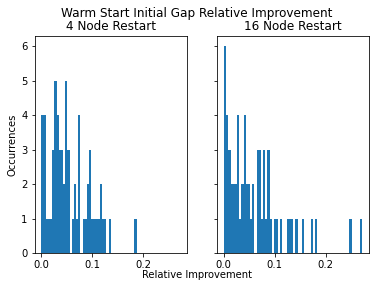
\includegraphics[width=.45\textwidth]{root_gap.png}}\hfill
		\subfloat[Relative improvement of warm start dual gap over cold start dual gap after evaluating as many nodes as the restart requirement]{\label{sf:restart_restart_gap}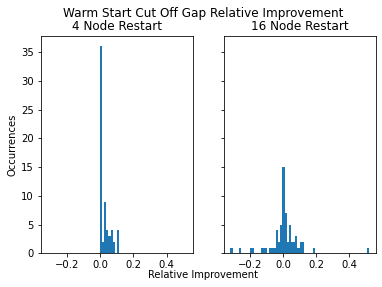
\includegraphics[width=.45\textwidth]{cut_off_gap.png}}\\
		\caption{Comparisons of the additional metrics}
		\label{f:restart_extra}
	\end{figure}
	
	\begin{figure}[h]
		\centering
		\subfloat[Relative improvement of warm start node evaluations over cold start node evaluations to reach 1\% primal-dual gap]{\label{sf:restart_node_evals}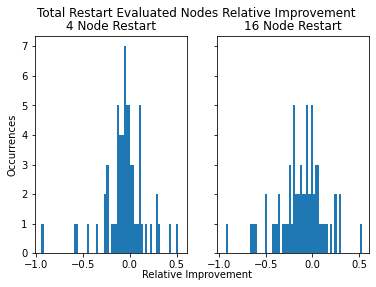
\includegraphics[width=.45\textwidth]{node_evals.png}}\hfill
		\subfloat[Relative improvement of warm start run time over cold start run time to reach 1\% primal-dual gap]{\label{sf:restart_gap}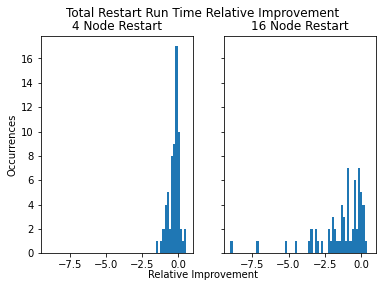
\includegraphics[width=.45\textwidth]{run_time.png}}\\
		\caption{Comparisons of main metrics}
		\label{f:restart_main}
	\end{figure}
	
	As we can see in Figure \ref{f:restart_main}, we worsen in both nodes evaluated and run time in most cases. We interpret this as the CGLP cuts we carry over from the initial solve to the warm start is not being helpful for improving the performance. We believe this to be the case as generating many cuts from the CGLP is more likely to be helpful as the extra cuts will further reduce primal-dual gap. We do see some promise in using CGLP cuts in Figure \ref{f:restart_extra} since the single cut we can generate from the initial solve does result in initial improvements in the dual gap. This leads us to believe that having a cut generating method where we could create CGLP cuts after bounding each node might be of great benefit to us. In a future version of this work, we will detail more what improvements we get from doing so.
	
	\section{Dual Decomposition for Stochastic MILP's}\label{s:stochastic}
	
	\subsection{Extension from Single Solve MILP}
	
	\subsection{Warm Starting Approach}
	
	\subsection{Numerical Results}
	
	\section{Branch and Price}\label{s:bnp}
	
	\subsection{Extension from Single Solve MILP}
	
	\subsection{Warm Starting Approach}
	
	\subsection{Numerical Results}
	
	\section{Multi-Objective MILP}\label{s:mom}
	
	\subsection{Extension from Single Solve MILP}
	
	\subsection{Warm Starting Approach}
	
	\subsection{Numerical Results}
	
	\section{MINLP}\label{s:minlp}
	
	\subsection{Extension from Single Solve MILP}
	
	\subsection{Warm Starting Approach}
	
	\subsection{Numerical Results}
	
	\section{Real-Time MILP}\label{s:rt}
	
	\subsection{Extension from Single Solve MILP}
	
	\subsection{Warm Starting Approach}
	
	\subsection{Numerical Results}
	
	\section{Serialized Local Search Primal Heuristic}\label{s:sls}
	
	\subsection{Extension from Single Solve MILP}
	
	\subsection{Warm Starting Approach}
	
	\subsection{Numerical Results}
	
	\section{Conclusion}\label{s:conclusion}
	As it stands currently, we need to finish developing working versions of all four warm starting techniques we listed in section \ref{ss:approach}, as having cut generating methods after bounding a node is still a work in progress. Further, we need to optimize each technique to be efficient to give us the best comparison to cold start run times as we can get. Lastly, we then need to implement a solve method for what remaining problem subclasses we want to test and repeat the experiment outlined in section \ref{s:eval}. After doing that, we hope to conclude with how effective warm starting is for each problem subclass we test and what further research directions remain.
	
	\newpage
	
	\bibliographystyle{plainurl}
	\bibliography{reference}
	
\end{document}